\documentclass{article}
\usepackage{lmodern} % Latin Modern Font
\usepackage[T1]{fontenc}
\usepackage{amsfonts} % \mathbb
\usepackage[margin=0.5in]{geometry}
\usepackage[utf8]{inputenc}
\usepackage{graphicx}
% \graphicspath{{images/}}
\usepackage[backend=biber]{biblatex}
\usepackage{amsmath}
\usepackage[makeroom]{cancel}
% \usepackage{auto-pst-pdf}

% \usepackage{hyperref}
% \usepackage{hypcap}
% \DeclareMathOperator{\sign}{sign}
% \hypersetup{
%   colorlinks=true, 
%   allcolors=black,
%   pdfauthor={Carlos Henrique Tarjano Santos},
%   pdftitle={Robust Digital Envelope Estimation Via Geometric Properties of an Arbitrary Real Signal}
% }

\bibliography{Compression}

\usepackage{authblk}
\title{Title}
\author[1]{Carlos Henrique Tarjano Santos}
\author[2]{Valdecy Pereira}
\affil[1]{(corresponding author, carlostarjano@id.uff.br) Department of Production Engineering, Universidade Federal Fluminense, Rua Passo da Pátria, 156, Campus Praia Vermelha, Bloco D - sala 309, São Domingos, Niterói, RJ, Brasil, CEP: 24.210-240}
\affil[2]{Department of Production Engineering, Universidade Federal Fluminense, Rua Passo da Pátria, 156, Campus Praia Vermelha, Bloco D - sala 309, São Domingos, Niterói, RJ, Brasil, CEP: 24.210-240}



\begin{document}

\maketitle

\begin{abstract} % ≅ 250 words  
% Clear and simple miniature version of the paper
% Self-contained
% Past tense for the current study
% Present tense to refer to stablished facts

% Background (What is already known about the subject)
Sample based virtual instruments are the de facto standard for the emulation of real word acoustic instruments. Nevertheless little attention is given to the encoding of the samples used in those instruments; in fact, lossless containers like wav or proprietary formats are common, pushing the on disk size of those libraries to sizes exceeding the gigabytes.
% Motivation (Why do we care about the problem and the results?) 
This renders the most realistic digital instruments inaccessible in many but the most high-end hardware; controllers, like electronic drum kits and controller keyboards and even less robust personal computers might encounter problems implementing those software.
% Problem | Objectives (What problem is the paper trying to solve?) (Scope)
We propose a lossy compression algorithm tailored specifically to highly uniform sounds, as those present in these instruments, due to the nature of the sounds, highly redundant, substantial improvements can be obtained, with minimal quality loss.

% Methods | Procedure | Approach (What did you actually do to get your results?)

% Results | Findings | Product (what did you learn | invent | create?)

% Conclusions | Implications (What are the larger implications of your findings)
The method, being physically informed, also serves as base 
lends itself well to machine learning, as the sound can be represented by an evolving waveform over time (pseudo-cycles)

\end{abstract}

{\bf Keywords:} 


\section{Introduction} % ≅ 500 words
% ≅ 10\% of the text
% broad to specific
% show that the research question is clear, concise, and worthy of study.
% allow the reader to understand the rest of the paper without referring to previous publications on the topic
% What did you do?
% conclusions

% Opener sentence (Question | Assertion | Intriguing Revelations)
Many of the proposed benefits of an electronic drumkit, like portability and practicity for example, are compromised when, to obtain a realistic sound on par with its acoustic counterpart, the output of the drumkit has to be processed in another piece of hardware, such as a personal computer.

The same is true for digital pianos, where models providing realistic sounds are many times more expensive than entry level models, owing in great part to the additional storage needed.

This transforms the instrument in a mere controller or practice aid, robbing it of characteristics that provide the personality of the conventional instruments, such as a particular timbre.

Domain specific compression algorithms and codecs exist in many areas. \textcite{2016ChenCompressing} for example, presents a scheme for compressing convolutional neural networks, while \textcite{2014CanovasLossy}, besides revising existing methods, proposes two lossy schemes for the compression of quality score data of genomic sequencing. 

More recently, the work of \textcite{2019CalhounExploring}, explores the benefits of specific lossy compression algorithms in the context of checkpoints of computational simulations that are stored between simulation sessions.

Regarding sample based digital musical instruments, to the best of the authors' knowledge, no such specialized algorithms exist. Those signals, being highly uniform, offer an opportunity for compression that is not present in most general sounds and remain largely unexplored.

This tendency arises in part from the marketing strategy of the vast majority of those products, where the sheer size of the library is advertised and seems to be sold as an equivalent of quality and versatility. An overall prejudice against compressed formats in general from the part of the music productions community supports this distorted view.

% Literature review | Brief Context of Prior Research
In that scenario, the work of \textcite{2019BlauRethinking} and, more recently, \textcite{2020O’GradyRethinking} are paramount in shedding light to the potential misconceptions permeating the opinion about lossy codecs, albeit from very different standpoints.

The first authors argue, from a technical point of view that perceptual quality metrics should be favored over metrics naively based on the mathematical aspect of Shannon’s rate-distortion theory \parencite{Shannon_1948}, the most popular metrics currently used in the assessment of lossy compression codecs. 

The second work analyses the problem from a somewhat political viewpoint, arguing that at last some of the criticism directed to the MP3 standard and lossy codecs in general is meant to stablish a symbolic capital in the face of the crescent struggle between established recording labels and alternative channel of music diffusion, such as streaming services.

% put your research in the context of other research
Nevertheless, research in data compression in general continues with recent efforts in reviewing the advancements of the field in general presented in \textcite{2021Jayasankarsurvey}. Account of the research in more specific areas, such as video \parencite{2019LaudeComprehensive} and image \parencite{2014RehmanImage} were also produced recently.

Concerning sound lossless audio compression research seems to be lagging when compared to lossy approaches; \textcite{2001HansLossless} suggested that a limit was about to be reached.

New technologies such as 3D, immersive audio has propelled specific compression algorithms, such as the one presented in \textcite{2021HuAudio}. The renaissance of neural networks led to interesting results, such as the use of GANs as presented in \textcite{2018HuangBandwidth}.


The ACER codec, as presented in \textcite{2014CunninghamData} offers an unconventional approach to compression, in that it identifies redundant pieces in a signal that are indexed in a dictionary. The results seems to be satisfactory from a perceptual standpoint, in comparison to MP3 and AAC codecs \parencite{2019CunninghamSubjective}. 


  % Nature and scope of the problem investigated
  % give them a framework for understanding it
  % What is the problem to be solved?
  % Are there any existing solutions?
  % Which is the best?
  % What is its main limitation?
  % What do you hope to achieve?

% Restate Your Question as Something Not Known or Fully Understood by Prior Research
  % identify the gap in the literature
  % use but, however, etc…

% State the Significance of Your Question
  % make readers understand why they should read your report

% State Your Claim | Objective | Hypothesis
  % should clearly relate to the information gap
  
% brief outlook on the structure of the paper

\section{Methodology} % ≅ 1000 words
  % How did you do it?
  % Justify choices
  % Describe the work so as people can reproduce it

% Overview of methods
A continuous or discrete signal, as long as it is at least pseudo periodic, can be interpreted as succession of consecutive waveforms, each one representing a (pseudo) cycle of the wave. In the case of perfectly periodic signals, those waveforms are identical and we need only the definition of one waveform to characterise the whole signal.in pseudo periodic waves, On the other hand there are potentially variations between pseudo cycles, that must be accounted for. If the wave is sufficiently well behaved, as is the case with most sound arising from accoustic phenomenons, these changes can be attributed to variations in both the amplitude of the waveform and its length


Starting with an initial estimate of the waveform of the signal being processed, one can identify the pseudo cycles of a signal by convolving the estimated waveform with the signal. The process can be made computationally efficient by considering some characteristics of the wave.

% Restate the purpose of the work

% Essential background information

% Relate to other studies

% Indicate where problems occurred



\section{Results} % ≅ 3000 words
  % What did you find?
  % Use figures, tables, etc.
  % Clearly and simply stated.

We compare the results of the algorithm here presented with some of the most popular codecs.

The first format we compare to is the popular MP3, the third layer of MPEG-1/2 specification, proposed in 1992 \parencite{2018BritanakAudio}. Despite being technically superseded by the newer MPEG-2 AAC \parencite{1999BrandenburgMP3}, finalized five years later, with which we also compare, its ubiquity makes the comparison crucial.

besides

The opus format was chosen, as, with the ACC and MP3, those are considered the most advanced \parencite{2019LaudeComprehensive} and popular \parencite{2018KwanObjective}

% Revisit purpose and methods

% Overview of results

% Key results in details

% Comparison with results in other works

% Comparison with predictions

% Problems with results

Since the average waveform is used to encode the specificities of the wave, signals where there are signficant variations in the sape of the waveform are naturally ill suited for compression with the presented algorithm. This limitation can be mitigated with a pre processing step where the waveform is segmented based on the overal shape of the waveform

noise

% Possible implications

\section{Discussion} % ≅ 2000 words

% Put results into a broader context.
While presenting an efficient algorithm to compress sufficiently well behaved signals, with immediate applications in the digital musical instrument industry, this work presents a new framework for representing pseudo periodic waves that can be extended in inumerous ways, with the help of both traditional and experimental methods.

While we simply consider the average waveform when encoding the compressed wave, more sofisticated representations can be used. The average waveform can be further compressed via a parametric representation.

% specific to broad

% What does it all mean?

% an interpretation of how each of the experiments supported your central hypothesis

% add in supporting findings from the literature

% what principles have been established or reinforced

\section{Conclusion} % ≅ 250 words
  % leave readers with a clear idea of your claim
  % make readers understand its importance
  % suggest further research
  stereo
  perceptual metrics
  % how the work advances the field?
  % significance and implications of the results
  % implications for broader application
  % research opportunities

% Restate Your Claim

% Point Out: New Significance | Practical Application | New Research


% \begin{figure}[ht!]
%   \centering
%      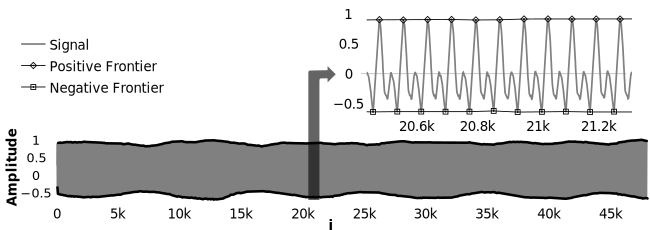
\includegraphics{images/01signalenvelope.pdf}
%   \caption{A discrete wave of the singing voice of an alto singer. The black lines are the frontiers; in the detail view, it can be seen that each region between two diamonds comprises a pseudo-cycle, as defined by the points belonging to the upper frontier. Similarly, two adjacent squares delimitate a pseudo-cycle, from the standpoint of the lower frontier.}
%   \label{fig:signalenvelope}
% \end{figure}



\printbibliography % 20 ⇔ 60 itens

\end{document}
